\section{Exact certificates, external reproduction, and unsuccessful searches}
\label{exp:section}

The experimental program serves two purposes: producing concrete coordinate
witnesses for lower bounds, and identifying which proposed general arguments
survive exact checks. These purposes require different standards of evidence.
A successful coordinate witness proves an existential lower bound at its
specified order. A failed search ordinarily proves neither an upper bound nor
the nonexistence of a better construction. This section records both positive
and negative outcomes without merging their logical scopes.

\subsection{From a numerical proposal to an exact geometric witness}

The stored coordinates use the convention $a_ix+b_iy=c_i$, with rational or
integer coefficients. Each line is normalized to a primitive integer triple.
Pair intersections are computed as homogeneous integer triples, normalized
with a positive final coordinate. Consequently, collinearity, concurrence,
parallelism, and comparisons along a supporting line can all be tested without
floating-point tolerances.

Two independently implemented counters are used. The first sorts the distinct
intersection vertices on each line and constructs the graph of elementary
bounded segments; a three-cycle supported by three different lines is a
triangular cell. The second enumerates support triples and tests whether every
other line has a common weak sign at their three vertices. Nonzero area and
the distinction between open interiors and boundaries are checked explicitly.
Where a complete independent verification is reported, both counters agree on
the triangle set, not merely on a rounded area or a visual estimate. The Lean
geometric soundness theorem provides a third, logically separate link from
accepted coordinate predicates to real affine triangles.

Numerical optimization is used only to propose coordinates or rank candidate
chambers. A proposal is rationalized and recounted before promotion. In the
phase/chart experiments, progressively finer integer scales were accepted only
when the entire exact triangle set and simplicity were retained. Such a finite
acceptance does not prove that an arbitrary rounding of an irrational
construction is valid. The real all-order theorem for $\G$ has its own
determinant, trigonometric, and counting proof.

The released catalog contains 138 distinct promoted coordinate identities.
Several identities can occur at the same order and triangle count, and an
identity may have several repository source paths. Thus 138 is a catalog size,
not a count of new records or independent discoveries. The complete catalog
in Table~\ref{exp:catalog} includes simple versus nonsimple status, provenance
collections, and coordinate-hash prefixes; its machine-readable companion
records full hashes, source paths, and theorem modules. The finite Lean
certificates use native evaluation where indicated. This trust boundary is
broader than that of the universal construction, whose proof uses only Lean's
standard logical axioms.

\subsection{Finite improvements relative to the retained collection}

The phase and affine-chart work raised the preceding saved values at eleven
orders:
\[
\begin{array}{c|rrrrrrrrrrr}
n&39&47&48&51&53&54&55&59&60&99&195\\\hline
\text{previous}&469&690&720&817&884&918&954&1102&1140&3169&12481\\
\text{current}&470&691&721&818&885&919&955&1103&1141&3170&12482
\end{array}
\]
Each row is an improvement over the project's preceding retained coordinate
catalog. The underlying trigonometric family is due to
F\"uredi--Pal\'asti~\cite{furedipalasti1984}; these comparisons do not establish
numerical first priority. The general formula $\G$ now explains all eleven
displayed counts. The first projective search reached $47:691$ after 11,264
proposals; the subsequent exposed-cap description replaced that search by a
direct construction and an all-order proof.

The earlier OEIS-attributed values $28:238$, $30:275$, and $34:357$ remain
independently certified~\cite{oeisA006066,zarzuelo2026}. The drawings in this
paper render the currently retained exact witnesses, obtained by exterior
extension of retained odd-order inputs. They are not asserted to be literal
reproductions of the March diagrams. Likewise, the historical inventory in
Table~\ref{exp:historical} preserves earlier outputs without upgrading every
original derivation to a completed general theorem.

The current strongest saved simple and classical coordinate counts for every
$3\leq n\leq60$ appear in Table~\ref{exp:finite-table}. An absent entry in the
explicit OEIS table is recorded as a dash. Absence from that table is not
evidence that a value is absent from the literature; conversely, a coordinate
certificate does not establish optimality without an upper theorem covering
the same arrangement class.

\subsection{Independent reproduction of external constructions}

The current Parpalak--Utkin coordinate gallery~\cite{parpalakutkin2026} supplied
exact witnesses at
\[
\begin{gathered}
8:15,\quad14:54,\quad20:117,\quad26:204,\quad32:315,\\
36:402,\quad38:450,\quad42:553,\quad46:667,\quad50:792.
\end{gathered}
\]
Both independent counters reproduced their triangle sets. These witnesses
retain their source attribution; in particular, the eight-line numerical
value has older discovery priority than the coordinate gallery. Their addition
to this repository improves its verified coverage, not the discoverer's
claim to the numbers. The inspected gallery snapshot is commit
\texttt{feae4f5571a988a3ed45bd26a36259ebb7d7d3d2}.

All fifteen of Andrea Maiorana's published $14:54$ coordinate
configurations~\cite{maiorana2026} were also independently checked. Fourteen
have exactly two triple points, and one has four; none has a parallel pair.
The source snapshot is commit
\texttt{e47c7cfd9661e54d29befb83118bf83d5f804028}. Its CC BY 4.0 licence,
original coordinate files, and source attribution are retained. Added wrappers
record counts and verification metadata. This reproduction imports no claim
that a simple-arrangement upper theorem applies to these nonsimple witnesses.

These examples also expose a concrete limitation of smoothing. In Maiorana's
first example, the triple supports are $\{0,4,10\}$ and $\{0,11,12\}$.
Independently shifting the offsets of lines 4 and 11 by $\pm1/1000$ realizes all
four local resolution choices while preserving every originally nonzero
determinant sign. The resulting triangle counts are $52,52,53,52$, all below
54. Thus the proposed nondecreasing local smoothing strategy fails even when
the local sign choices are independently realizable by straight lines. The
argument identifying these sign choices with all sufficiently small local
resolutions is an ordinary finite sign-stability argument, not a completed
Lean theorem.

For the gallery's collinear-core examples at orders
$8,14,20,26,32,38,50$, all 132 recorded local resolutions were realized by
exact private-line offsets. Their respective best simple counts were
$14,51,114,203,313,448,791$. In particular, a universal claim that resolving
such a core loses at most one triangle is also false. Figure~\ref{fig:external-comparison}
separates these finite obstructions from any general upper-bound assertion.

\begin{figure}[tbp]
  \centering
  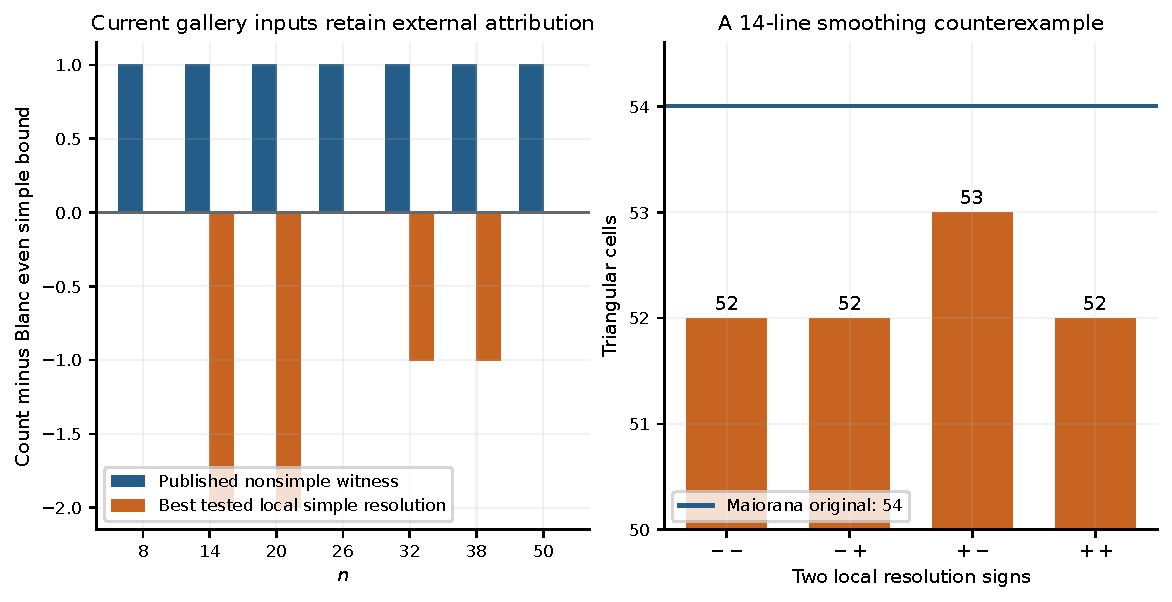
\includegraphics[width=\textwidth]{figures/external-comparison.pdf}
  \caption{Exact local-resolution tests on attributed external constructions.
  Left: Parpalak--Utkin gallery witnesses and their best tested simple local
  resolutions, measured relative to Blanc's even simple-arrangement polynomial;
  the eight-line value has older priority. Right: all four local resolutions of
  Maiorana's two-triple-point $14:54$ example. The original arrangements are
  nonsimple, so exceeding the simple polynomial is consistent. These are
  smoothing obstructions, not upper bounds for the classical problem.}
  \label{fig:external-comparison}
\end{figure}

\subsection{Projective charts, algebraic curves, and chamber searches}

Projective geometry provides a useful global neighborhood: changing the line
at infinity moves all lines together and may bound formerly unbounded
triangular faces. It can also lose bounded cells. For the exact saved
$81:2132$ and $161:8532$ hybrid arrangements, the projective triangular-face
census already equals their bounded-cell count; a chart change alone cannot
increase those particular counts.

Exact rational linear-arithmetic searches give sharper restrictions for some
fixed configurations. The nine-line half-phase rational arrangement has 21
projective triangular faces, but the recorded QF\_LRA solver result rules out a
chart retaining all 21. Similar fixed-seed tests find no gain for the tested
half-phase arrangements at $14,20,26,44$, and no chart retaining all 471
projective triangles of the saved $39:470$ witness. For a nonuniform cubic
48-line seed with 724 projective triangles, 2,903 exact linear-arithmetic checks
rule out 722 bounded triangles within the tested chart-retention formulation.
These are exact-solver results about specified rational seeds. Their UNSAT
certificates have not been independently checked in Lean, and they are not
global upper bounds at those orders.

The algebraic-curve direction tested both nodal-cubic angle perturbations and
torsion cosets on real elliptic curves. A larger projective face count did not
automatically produce a better affine construction. For the better two-real-
component elliptic examples, the projective, original affine, and best found
affine counts were respectively
\[
\begin{array}{c|rrrr}
n&42&48&54&60\\\hline
\text{projective}&550&724&922&1144\\
\text{original affine}&538&710&907&1127\\
\text{best found affine}&539&712&908&1129
\end{array}
\]
All fall below the corresponding retained affine bounds. The chart scans at
54 and 60 had 90-second limits. Numerical ranking and bounded running time
preclude a global nonexistence inference.

Oriented-matroid mutations and kinetic chamber sweeps addressed a different
limitation: moving inside a fixed projective type cannot create new
projective triangular faces. The mutation searches changed determinant signs,
using linear-programming realization where appropriate. Kinetic sweeps varied
many offsets, or both slopes and offsets, and visited concurrency events along
selected rays. Their event counts are not counts of all realizable order
types, and unsuccessful floating rays were discarded. Figure~\ref{fig:negative-searches}
records effort without treating heterogeneous search units as comparable
coverage measures.

\begin{figure}[tbp]
  \centering
  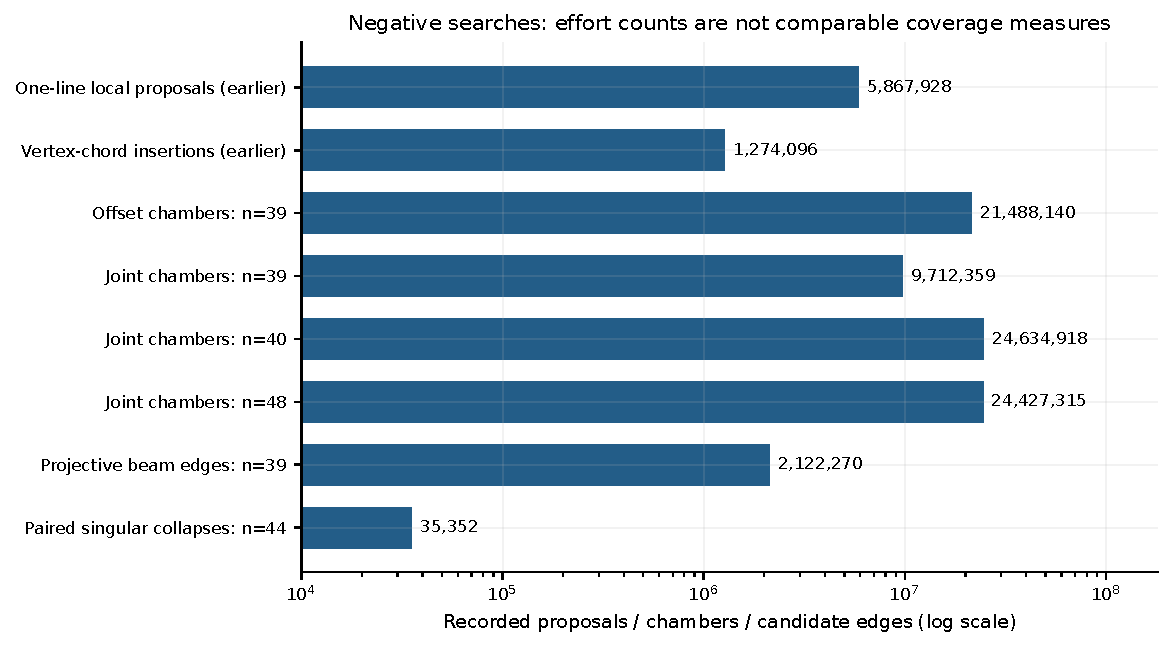
\includegraphics[width=\textwidth]{figures/negative-searches.pdf}
  \caption{Selected unsuccessful searches, with their recorded units.
  Proposal, chamber, and candidate-edge totals describe different search
  neighborhoods. They do not measure exhaustive coverage, justify an upper
  bound, or rank the mathematical promise of the methods. All proposed
  improvements would require subsequent exact geometric verification.}
  \label{fig:negative-searches}
\end{figure}

The final 39-line projective beam examined 2,122,270 candidate edges through
4,559 states without exceeding 470 affine or 471 projective triangles, even
at its combinatorial scoring stage. The 48-line LP walk accepted 471 mutations
out of 511 attempts and retained 721 affine and 724 projective triangles.
At 44 lines, singular-boundary searches included 35,352 paired collapses;
the retained beam checkpoint had 771 states and 446,422 candidate edges,
without exceeding 608. An unfinished round was discarded. These results
motivate a change of neighborhood or a structural argument rather than
repeating the same local searches.

Other bounded approaches included Fourier deformations (2,687,600 proposals
in one 39-line run), partial deletions from BBL constructions, and constrained
tangent-grid transfer by LP/MILP. The tested optimal 23-line chart transfers
did not admit a positive-margin realization on the desired grid; a constrained
near-optimal search gave 144 triangles, below a separately known compatible
145. None of these observations proves nonexistence of another compatible
seed or a different successful deletion pattern.

\subsection{A proved algebraic obstruction to tangent-grid transfer}
\label{exp:grid-obstruction}

The October search connects oriented-matroid sign constraints, linear
programming duality and exact algebraic number arithmetic. For the
reciprocal-coordinate lines $x-v_i y=a_i$, a prescribed determinant
sign becomes a strict linear inequality in the unknown reciprocal
slopes. Write
\begin{equation}
 D_{ijk}=(a_j-a_k)v_i+(a_k-a_i)v_j+(a_i-a_j)v_k.
 \label{exp:linear-determinant}
\end{equation}
Once the intercepts are fixed, feasibility is a linear sign problem,
even though the intercepts themselves are algebraic.

\begin{lemma}[Positive-dependence obstruction]\label{exp:farkas}
Let $A_i\in\R^d$ and let $\lambda_i\ge0$, with at least one
$\lambda_i>0$, satisfy $\sum_i\lambda_i A_i=0$. There is no $v\in\R^d$
with $A_i\mathbin{\cdot}v>0$ for every $i$.
\end{lemma}
\begin{proof}
Taking the scalar product with $v$ makes the left side a positive
weighted sum, but the assumed vector identity makes it zero. This
classical strict alternative is formalized by
\sourcefile{Kobon/StrictLinearCertificate.lean}{\lean{homogeneous_infeasible}}.
The formal theorem also provides an affine form for nonhomogeneous
strict systems.
\end{proof}

Set $t=\tan(\pi/20)$. Its exact algebraic specification is
\begin{equation}
 p(t)=t^4-4t^3-14t^2-4t+1=0,
 \qquad \frac3{20}<t<\frac{17}{100}.
 \label{exp:quartic}
\end{equation}
The quintuple-angle identity with $\tan(5\pi/20)=1$ gives
$(t-1)p(t)=0$; the interval excludes $t=1$. Monotonicity on the interval
identifies the intended root. \lean{BBLTangentAlgebra} proves the
quartic, root interval and uniqueness; \lean{BBLTangentValues} proves
that its explicit cubic power-basis expressions are the actual nine
values $\tan(k\pi/20)$ for $1\le k\le9$. Thus replacing trigonometric
numbers by algebraic expressions does not insert a numerical guess.

Use the actual 20-intercept grid
\[
 a_j=\begin{cases}
 -\tan((9-j)\pi/20),&0\le j<9,\\
 -\varepsilon,&j=9,\\
 \varepsilon,&j=10,\\
 \tan((j-10)\pi/20),&11\le j<20.
 \end{cases}
\]
The following ten prescribed signs are impossible.

\begin{theorem}[One exact tangent-grid obstruction]
\label{exp:actual-grid-obstruction}
For every real $\varepsilon$ and every real vector
$(v_0,\ldots,v_{19})$, at least one row of
Table~\ref{exp:ten-signs} fails the strict inequality
$s_iD_{j_i k_i\ell_i}>0$.
\end{theorem}

\begin{table}[tb]
\centering\small
\begin{tabular}{@{}cll@{}}
\toprule
Support triple & $s_i$ & Positive multiplier $\lambda_i(t)$\\
\midrule
$(0,6,15)$ & $-1$ & $-20t^3+120t^2+300t-40$\\
$(0,7,13)$ & $+1$ & $-8t^3+24t^2+96t+8$\\
$(0,8,14)$ & $-1$ & $-45t^3+205t^2+555t-35$\\
$(0,13,19)$ & $+1$ & $-16t^3-6t^2+40t+2$\\
$(3,6,8)$ & $+1$ & $20t^3-100t^2-220t+100$\\
$(3,11,15)$ & $-1$ & $20t^3-120t^2-220t+200$\\
$(3,13,17)$ & $+1$ & $20t^3-150t^2-300t+130$\\
$(7,11,13)$ & $+1$ & $-60t^3+240t^2+860t+320$\\
$(8,14,17)$ & $-1$ & $-105t^3+455t^2+1275t-45$\\
$(8,15,19)$ & $-1$ & $36t^3-188t^2-452t+124$\\
\bottomrule
\end{tabular}
\caption{An explicit positive linear-dependence certificate. Indices are
zero-based intercept indices. The rows use eleven distinct intercepts
and avoid the two exceptional central indices. Each column of the
weighted signed coefficient matrix vanishes modulo $p(t)$.}
\label{exp:ten-signs}
\end{table}

\begin{proof}
For each row define $A_i$ to be the coefficient vector of $s_iD$ in
\eqref{exp:linear-determinant}. All ten displayed multipliers are
positive throughout $3/20<t<17/100$, by rational polynomial inequalities.
Using the proved power-basis expressions for the tangents, expand
$\sum_i\lambda_i(t)A_i$ one column at a time and reduce modulo $p(t)$.
Every column is zero. The two central columns vanish because none of
the ten supports uses indices 9 or 10. Lemma~\ref{exp:farkas} gives a
contradiction. The exact source contains the polynomial multiple of
$p$ for every nontrivial column, so the computation is reproducible
without a floating-point linear solver. The declarations
\proofref{Kobon/BBLGridObstruction.lean}{240}{\lean{actual_grid_infeasible}}
and
\proofref{Kobon/BBLGridObstruction.lean}{263}{\lean{actual_grid_orientation_impossible}}
prove this for the actual tangent grid using only standard logical
axioms.
\end{proof}

This excludes one explicit orientation system with arbitrary reciprocal
slopes and every real central parameter. It does not classify all
21-line arrangements. An independent exact interval Gaussian-elimination
check also proves persistence under independent perturbations of radius
$10^{-3}$ on the eleven used intercepts. That robustness calculation is
external exact evidence, not part of the Lean theorem above.

\subsection{The full supplied affine-class obstruction census}
\label{exp:affine-census}

Parpalak--Utkin's enumeration separates projective and Euclidean
classes~\cite{parpalakutkinEnumeration2026}. This distinction changed
the scope of the search. The first checker verified 366 exact polynomial
certificates for eighteen supplied projective representatives on
$0<\varepsilon<1/25000$. A projective representative alone does not
exhaust its affine cases: a choice of infinity support matters. That
initial census was therefore insufficient for a complete affine claim.

The corrected checker expands all 236 supplied Euclidean classes and
all 21 choices of distinguished support. It validates 3,765 exact
polynomial dependencies and 15,060 reflected or reoriented variants,
covering all $236\cdot21=4,956$ class/support cases with no missing case,
for
\begin{equation}
 0<\varepsilon<1/2{,}000{,}000.
 \label{exp:census-interval}
\end{equation}
Every certificate is a positive linear contradiction of the form above,
so it excludes arbitrary, even parameter-dependent, reciprocal slopes.
The small positive interval is a uniform bound for this finite corpus;
it is not the unrestricted all-real parameter assertion proved for the
single ten-sign representative.

The logical dependencies remain separate. The completeness of the
classification is supplied by Parpalak--Utkin and its dataset. The
present independent checker validates the listed exact certificates,
the class/support coverage and the explicit symmetries. It does not
rerun their full enumeration inside Lean. The resulting exclusion of a
perfect 21-line seed on this prescribed saturated grid and interval is
therefore computer-assisted mathematics with an external classification
input. Only Theorem~\ref{exp:actual-grid-obstruction} is a complete
representative Lean obstruction. Other grids, larger seeds, nonsimple
arrangements and other construction methods remain unrestricted by this
census.

\subsection{New bounded searches and their exact outcomes}

The October work also tested finite neighborhoods selected to change
features that the earlier chart-only searches preserved. None produced
a new numerical lower-bound record. The exact positive and negative
results are summarized below; completed enumeration of a listed
neighborhood does not imply enumeration of all arrangements.

\begin{table}[tb]
\centering\small
\begin{tabularx}{\linewidth}{@{}P{0.29\linewidth}XP{0.24\linewidth}@{}}
\toprule
Search & Result & Limitation\\
\midrule
Deletions from a 49-line seed & Best retained values $48:721$, $47:677$,
$46:637$, $45:598$. & The tested deletion neighborhood only.\\
57-line MILP deletions & Incumbents $56:990$, $55:939$, $54:887$,
$53:837$. & Timed runs; incumbents are not proved maxima.\\
All 9,180 tested chords of a 17-line seed & Best 18-line output has 93
triangles. & Chords of one seed.\\
407,253 vertex-pair insertions at 43 lines & Best 44-line output has
607 triangles, below retained 608. & The stated insertion neighborhood.\\
Singular 16-to-18 insertion & Best recorded count 89. & No global
exclusion.\\
39-pseudoline straightening & Exact realizations with 353 and 358
triangles. & Neither a record nor a proof of nonstretchability.\\
Perfect 21-line grid fit & Exact affine-class obstruction census. & The
prescribed grid, interval and supplied classification.\\
49-line grid fit & Uniform 767-cell certificate and full visible boundary.
& Exact external certificate; full Lean base pending.\\
\bottomrule
\end{tabularx}
\caption{The added research directions and their actual conclusions.
The 49-line positive result is compared with its known BBL numerical
family in Section~\ref{fam:seed49}.}
\label{exp:october-searches}
\end{table}

The methodological connection to recent automated mathematical search
is a separation of proposal, evaluation and proof, also emphasized by
Georgiev, G\'omez-Serrano, Tao and Wagner~\cite{georgiev2025}. Here a
numerical optimizer proposes a coordinate or dual vector; exact
arithmetic certifies the finite claim; the symbolic construction or
obstruction explains which statements hold uniformly. Their paper is
methodological context, not evidence that Kobon has already been solved.
The author's other construction projects motivated preserving an
iterable invariant and exploiting symmetry orbits; none of their
unrelated theorems is imported as a Kobon lemma.

\subsection{Reproduction and presentation audit}

The research registers preserve source snapshots, experiment scripts, seeds,
parameters, checkpoints, and exactness limits~\cite{zarzueloRepository}. The
paper's figures are original vector renderings, not copied source figures.
The generator \texttt{paper/scripts/generate\_figures.py} reads the research
data without modifying it and exports PDF figures, PNG previews, LaTeX tables,
and machine-readable rendering data. The figure manifest records input-file
hashes and the mathematical status of each caption. Geometric views recompute
their exact triangle lists before converting coordinates to floating point
for display. Cropped detail panels and independent affine axis rescaling are
explicitly labeled; lengths and angles are not inferred from those views.

The appropriate experimental conclusion is therefore selective. Exact
coordinates have strengthened the retained lower-bound envelope and revealed
specific failed construction rules. The successful universal advance comes
from replacing a numerical chart search by a geometric exposure proof and an
all-order count. The remaining negative searches narrow useful next steps,
but they do not solve the general optimization problem.
